\begin{tikzpicture}
  \node[anchor=south west, inner sep=0] (image) at (0, 0) {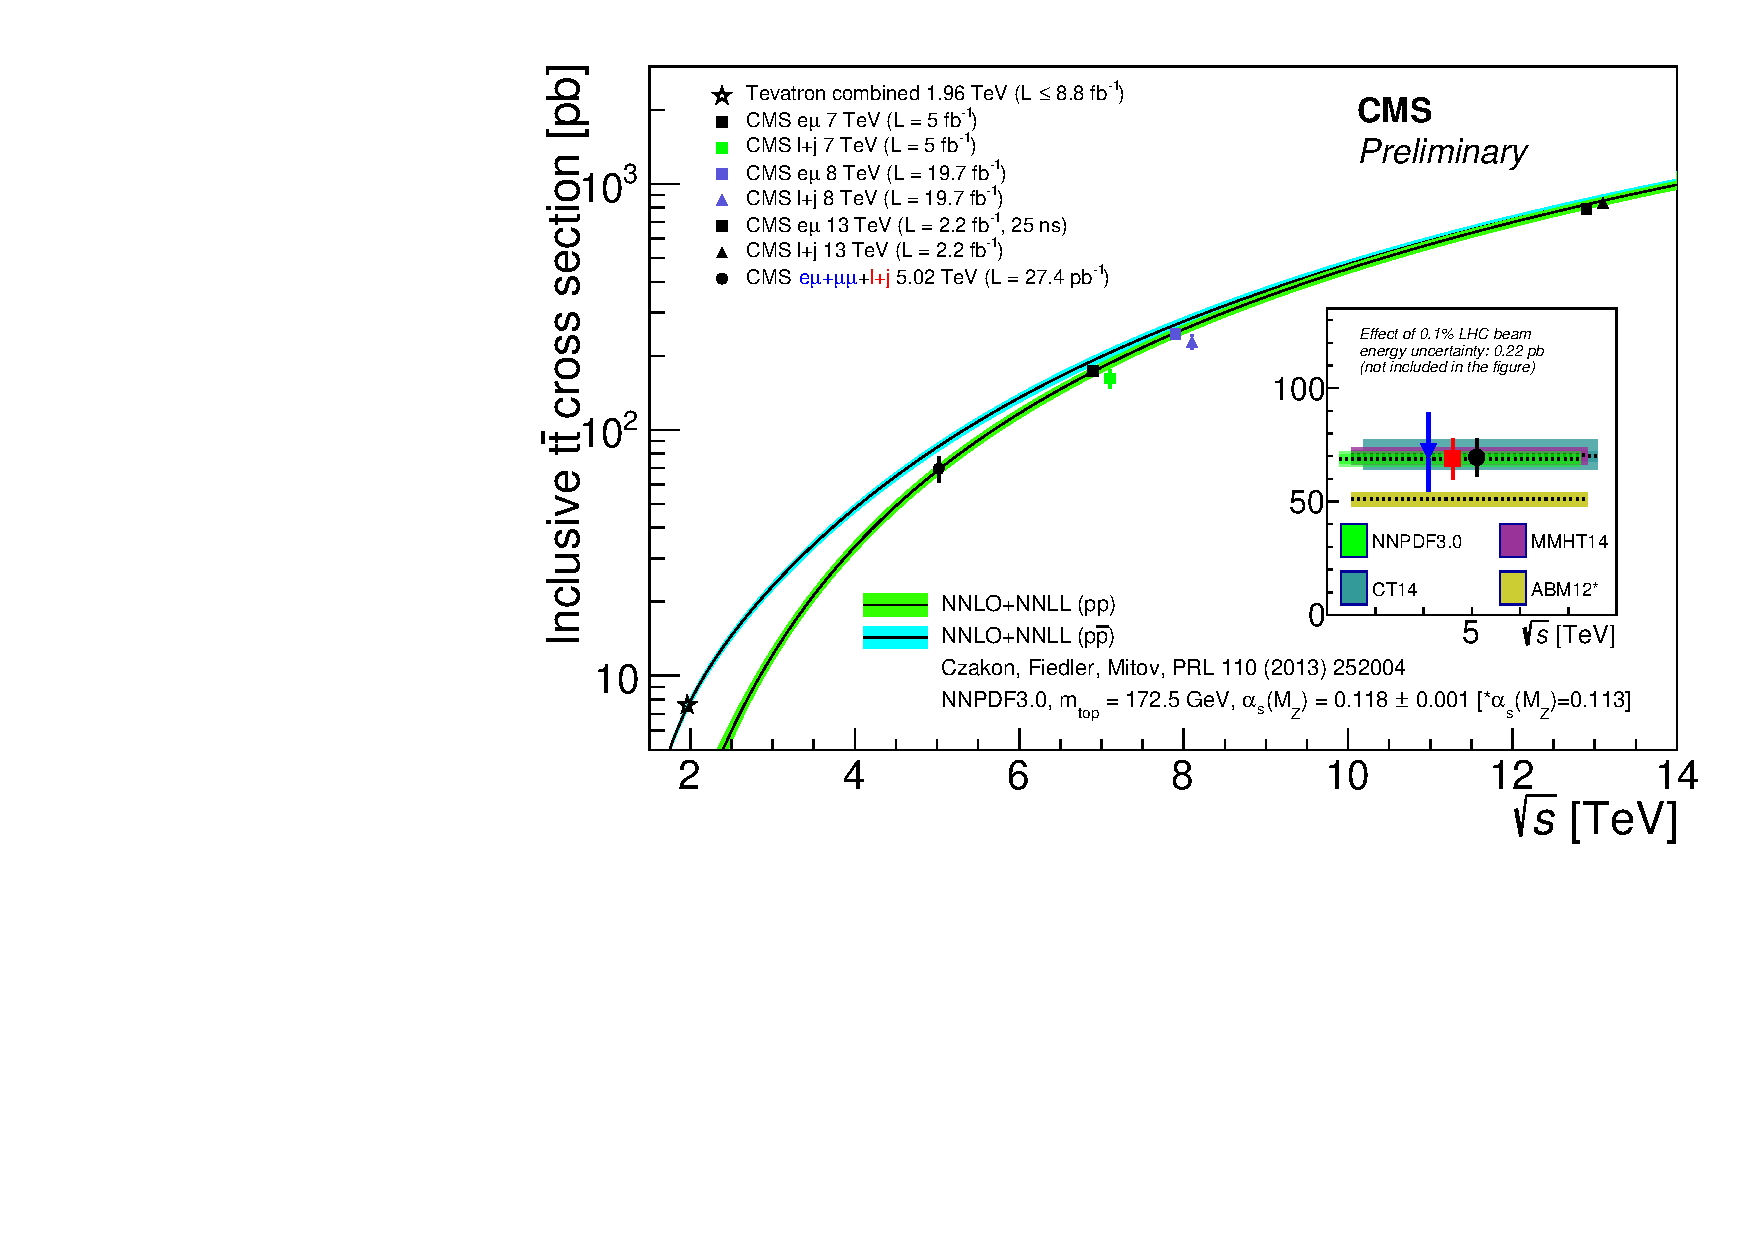
\includegraphics[width=\textwidth]{cms_ttbar_xsec_sqrts_spectrum}};
  \begin{scope}[x={(image.south east)}, y={(image.north west)}]
    % Grid to help find coordinates on the image
    % \draw[step=0.02, gray, very thin] (0, 0) grid (1, 1);
    % Box to cover axis labels
    \draw[thick, color=red!70] (0.345, 0.47) circle (0.4cm);
    % \path[fill=white] (0.02, 0.16) rectangle (0.18, 0.22) node [pos=0.5] {\footnotesize$\theta_{1}$};
  \end{scope}
\end{tikzpicture}
